%!TEX root = manual.tex
%===============================================================================
\chapter{Install the cross-compilation tools}\label{ch:Assignment2}

The aim is to get acquainted with the embedded computer board and to install and test the cross-compilation tools for GNAT that will be used to develop executable code for it.

\section{Cross-compilation tools}

The computer board will programmed in Ada. The GNAT cross-platform software development system will be used (figure~\ref{fig:cross}), where the student PC is the host platform and the SMT32 board is the target platform.

\begin{figure}[h]
            \centering{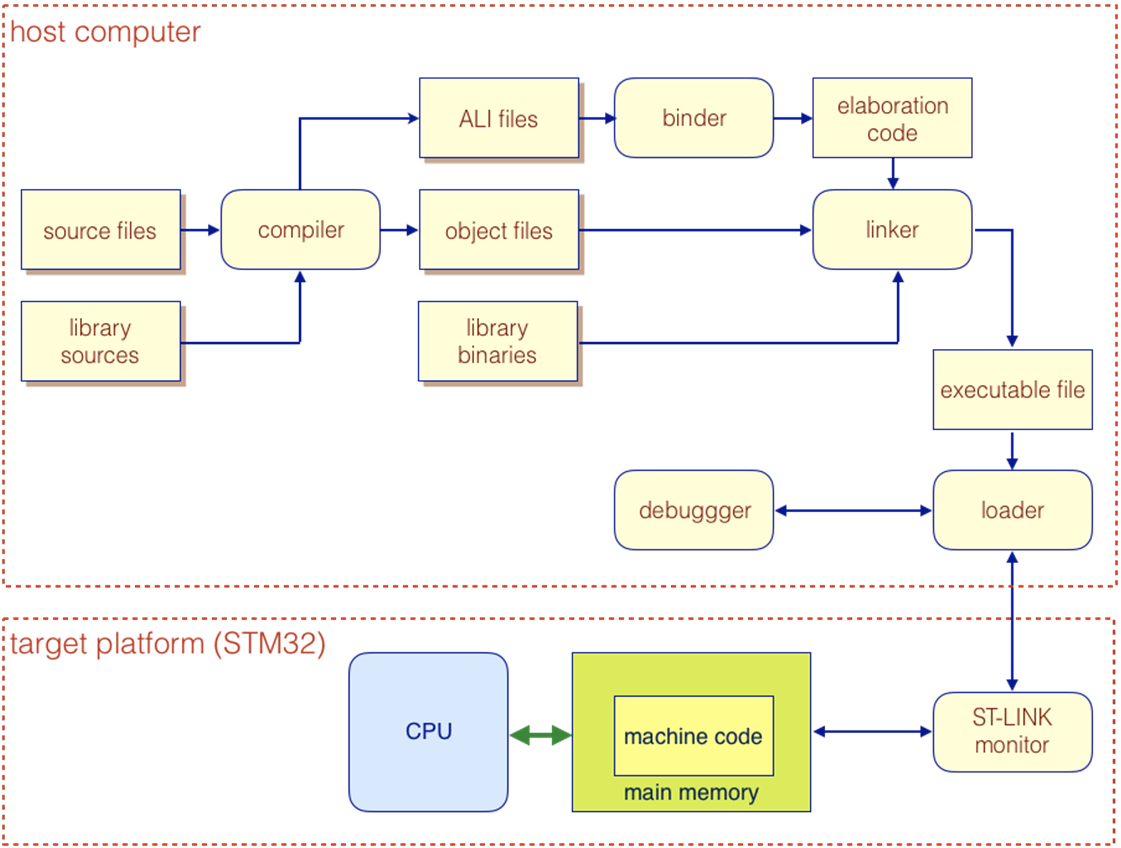
\includegraphics[width=\textwidth,keepaspectratio]{cross.png}}
            \caption{Cross-compilation and debugging system}
            \label{fig:cross}
\end{figure}

In order to compile a program, the compilation chain is run on the host computer to produce an executable file for the target computer. The executable is then loaded into the target memory, from where it can be run. A monitor program is preinstalled on the target board that supports loading and debugging from the host platform.

\section{Download and install GNAT ARM ELF}

GNAT ARM ELF is the cross-compilation chain to be used with the STM32F4 board. It can be downloaded from the same page as the native GNAT system, https://www.adacore.com/download/more, and there are installation packages for Windows, MacOS and GNU Linux available. The file {\tt README.txt} provides installation instructions, which are summarised as follows.
\subsection{Windows}
\begin{enumerate}
\item Select ARM ELF (hosted on windows64) and download the file\\
{\tt gnat-2021-20210519-arm-elf-windows64-bin.exe}
\item Run the file and follow the instructions.
\item You will also need to install the USB driver for the ST-LINK probe. To do so, go to \url{http://www.st.com/content/st\_com/en/products/embedded-software/development-tool-software/stsw-link009.html}, and click on {\tt Get Software}. Click on {\tt Get Software} under the {\tt Download} column of the table that shows up to obtain the driver. You will need to accept ST Micro's license agreement and enter your contact details. 
Once downloaded unzip the USB device driver and run the installer, accepting all the defaults.
\end{enumerate}
\subsection{MacOS}
\begin{enumerate}
\item Download the file {\tt gnat-community-2019-20190517-arm-elf-darwin-bin.dmg}
\item Open the dmg disk and execute the application inside it. In order to circumvent the system protection, control-click on the file and then click on ``open" in the emergent window.
\item You will also need the st-util,  st-flash, and st-info tools. You can download the binaries from 
\url{https://github.com/texane/stlink/releases/download/1.3.0/stlink-1.3.0-macosx-amd64.zip}. Unzip and copy the files in the bin directory to a directory in your {\tt PATH}. You may need to circumvent MacOS protection by executing the command:
\begin{verbatim}
	\$ xattr -d com.apple.quarantine path-to-executable-file
\end{verbatim}
\end{enumerate}
\subsection{GNU Linux}
\begin{enumerate}
\item Download the file {\tt gnat-2021-20210519-arm-elf-linux64-bin}
\item You will need to make the package executable before running it. In a command prompt, execute the following command:
\begin{verbatim}
     chmod +x path\_to\_the\_package.bin
\end{verbatim}
and then execute the package.
\item You will also need to install the stlink tools. In Ubuntu and Debian stlink must be installed from sources. Follow the instructions on \url{http://docs.adacore.com/live/wave/gnat\_ugx/html/gnat\_ugx/gnat\_ugx/arm-elf\_topics\_and\_tutorial.html\#linux}.
\end{enumerate}

The {\tt README.txt} file contains additional installation and execution instructions.

\section{Test your installation with an embedded program}

The next thing is to compile a run a simple embedded program. This program is only intended to test that the compilation chain and the ST-LINK tools have been properly installed.

Open GPS and do the following:
\begin{enumerate}
\item Create a new project by clicking on {\tt File} $\rightarrow$ {\tt New Project} ... in the top menu. Choose the {\tt STM324F compatible} $\rightarrow$ {\tt LED demo project template}.
\item	Choose a folder to deploy the project, e.g. OBDH\_LABS/LAB2. Set the project name to {\tt led\_demo} and the main name to {\tt main.} A window with a project including a number of source files will open.
\item	Right-click on the project icon on the left side area, and choose {\tt Project} $\rightarrow$ {\tt Properties} (figure 6). On the emerging window, select Embedded and change the Connection tool selector to st-util. Save the settings.
\item	Connect the STM32F4 board to the computer by means of a USB A / mini USB cable.
\item	Build the executable and load it into the board by clicking on the
\hbox{
\includegraphics[width=1.5em]{buildandload.png}} symbol in the tool bar (or select {\tt Build} $\rightarrow$ {\tt Bareboard} $\rightarrow$ {\tt Flash to board} on the top menu). You should see a number of compilation-related messages ending with ``Flashing complete. You may need to reset or cycle power".
\item	If everything is all right, you will see the LEDS on the board blinking in a circular pattern.
\item Download and install the Ada Drivers Library
The Ada Drivers Library is a set of Ada packages that make it easier to write software for embedded devices, including the STM32F4 microcontroller family and some demonstration boards. The source code can be found at \url{https://github.com/AdaCore/Ada\_Drivers\_Library}. To install the library, click on the green {\tt Clone} or {\tt download} button on the upper right side and then on Download Zip in the emerging window. You will get a zip archive in your downloads folder. Unzip the archive and move the resulting folder to your OBDH\_LABS folder. Rename the folder to {\tt Ada\_Drivers\_Library}, removing any trailing text.
\item Compile and run a test program with the Ada Drivers Library
\end{enumerate}
Open GPS and do the following:
\begin{enumerate}
\item Select {\tt Open} project on the welcome window. Navigate to .../OBDH\_LABS/\-Ada\_Drivers\_Li\-brary/\-examples/STMF4\_DISCO and open the project file: {\tt blinky\-\_f4disco.gpr}.
\item	Build the executable and load it into the board by clicking on the \hbox{
\includegraphics[width=1.5em]{buildandload.png}} symbol in the tool bar (or select {\tt Build} $\rightarrow$ {\tt Bareboard} $\rightarrow$ {\tt Flash to board} on the top menu). When the loading is complete, you will see the board LEDS blinking all at the same time.
\end{enumerate}

\section{Install MATLAB\texttrademark and Simulink\texttrademark}

MATLAB and Simulink will be used to generate C code from a Simulink model and 
to validate the system by Processor In the Loop (PIL).

UPM has a campus license available for students. \url{http://www.upm.es/sfs/Rectorado/Vicerrectorado\%20de\%20Tecnologias\%20de\%20la\%20Informacion\%20y\%20Servicios\%20en\%20Red/Servicio\%20de\%20Planificacion\%20Informatica\%20y\%20Comunicaciones/SW/MATLAB_UPM_Estudiantes.pdf} explains how to install MATLAB and Simulink.

In order to generate C code, the Embedded Coder toolbox and its dependencies must be installed.
